\chapter{Materials and Methods}
\section{Data selection}
For a Boolean network inference the data of a platform so-called Dialogue on Reverse Engineering Assessment and Methods (DREAM) - Challenge is used. The DREAM-Challenge is a non-profit, collaborative community effort consisting of contributors from across the research spectrum of questions in biology and medicine. This organization was built in 2006 and publishes crowdsourcing challenges with transparent sharing of data, thus everyone can participate the challenge. The DREAM-Challenge has partnered with Sage Bionetworks, which provide the infrastructure by Sage Bionetworks Synapse platform to get access to the open collaborative data analysis. Overall the DREAM-Challenge is a helpful instrument to get real-life data, comparing results and interact with other researchers all over the world, while contribute solutions to biological and medical questions.
Two DREAM-Challenges appear useful for this work. The first is the DREAM5- Network Inference Challenge (DREAM5) and the second the HPN-DREAM brest cancer network inference challenge (DREAM8)\citep{DreamChalleneg Homepage}. 

\subsection{DREAM5}
Living cells are the product of gene expression programs involving regulated transcription of thousands of genes. Gene expression programs depend on recognition of specific promoter sequences by transcriptional regulatory proteins. How a collection of regulatory proteins associates with genes across a genome can be described as a transcriptional regulatory network. This map of the transcriptional regulatory network describes potential pathways bacteria cells (S.aureus, E.Coli, S. cerevisiae) can use to regulate global gene expression programs \citep{Lee799}.
The DREAM5-Challenge states the challenge to infere a complete (genome-scale) transcriptional regulatory network for four organisms: in silico, S.aureus, E.Coli, S.cerevisiae. 

%-----> Zeigen wie das in silico data set gemacht wurde?

The data is yielded by genechip experiments, where mRNA is extracted from the samples, then reversetranscriped into more stable cDNA (complementary DNA), which is fluorescent labeled. Afterwards the cDNA binds to the complementary bases on the chip. Thus the DNA composition can be detected and it can be recognized wether a gene is active or not by the information of its transcript.
Just the gene expression profiles for the in silico network were derived from another platform so-called GeneNetWeaver \citep{GeneNetWeaver}.

%\begin{table}[h]
%\centering
%\begin{tabular}{ccccc} 
%\hline
%Network & Organism & TranscFactors & Genes & Chips\\
%\hline
%Network 1 &	in silico &	195 &	1643 &	805\\
%Network 2 & S.aureus  & 99  &	2810 &	160\\
%Network 3 & E. coli   &	334 &	4511 &	805\\
%Network 4 & S. cerevisiae &	333 & 5950 & 536\\
%\hline
%\end{tabular}
%\captionof{table}{Overview}
%\label{table:Table 1}
%\end{table}\\


\begin{figure}
\centering
%\setlength{\abovecaptionskip}{0pt}
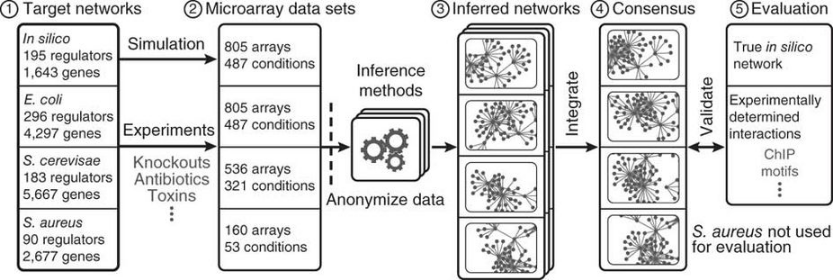
\includegraphics[width=0.8\textwidth]{./Bilder/assessment}
\caption[Interaction Graph]{\textbf{Assessment involved the following steps}Assessment involved the following steps }
%\setlength{\belowcaptionskip}{0pt} 
\label{fig:Fig.1.}
\end{figure}

In this challenge some experiments have pertubations in terms of gene deletion, overexpressed genes and  adding drugs to the system. Few experiments were done the same konfiguration several times. Some experiments are part of a time-series measurement and some are not,described in Figure 2.
For each network, a list of directed, unsigned edges had to be submitted ordered according to the participants confidence scores. 
The participants are given four microarray sets. In each set are three  tsv.-files  (tab-seperated values) with the gene expression data, chip-features and transcription factors.\\

\noindent\fbox{
    \parbox{\textwidth}{
\begin{flushleft}
\texttt{Network{\_}i{\_}\textbackslash{\_}expression\textbackslash data.tsv}\\
\texttt{Network{\_}i{\_}\textbackslash{\_}chip\textbackslash{\_}features.tsv}\\
\texttt{Network{\_}i{\_}\textbackslash{\_}transcription\textbackslash{\_}factors.tsv}\\
\end{flushleft}
    }
}


%where $i\in\lbrace 1,2,3,4\rbrace$

%\begin{center}
\begin{table}[H]
\scriptsize
\centering
\begin{tabularx}{\textwidth}{lllllllll} 
\hline\hline
Chip & Experiment &  Pertubations &  PertubationLevels &  Treatment &  DeletedGenes &  OverexpressedGenes &  Time &  Repeat\\
\hline \hline
1 & 1 &	NA & NA & NA & NA & NA & NA & 1\\\hline
2 &	1 &	NA & NA & NA & NA &	NA & NA & 2\\\hline
3 &	2 & NA & NA & NA & NA & NA & NA & 1\\\hline
4 &	2 &	P1 & 0.5 & NA & NA & NA & NA & 1\\\hline
5 &	2 &	P1 & 1.0 & NA & NA & NA & NA & 1\\\hline
6 &	3 &	NA & NA & NA & NA & NA & 0 & 1\\\hline
7 &	3 &	NA & NA & NA & NA & NA & 30 & 1\\\hline
8 &	3 &	NA & NA & NA & NA & NA & 60 & 1\\\hline
9 &	3 &	NA & NA & NA & G5 & NA & 30 & 1\\\hline
10 & 3 & NA & NA & NA & G5 & NA & 60 & 1\\\hline
11 & 4 & NA & NA & NA & G5,G8 & NA & NA & 1\\\hline
12 & 5 & P2,P3 & NA & NA & NA & G4 & NA & 1\\\hline
13 & 5 & P2,P3 & NA & 1 & NA & G4 & NA & 1\\
\hline
\end{tabularx}
\captionof{table}{Chip information}
\label{table:Table 2}
\end{table}
%\end{center}

The \texttt{Network{\_}i{\_}\textbackslash{\_}expression\textbackslash data.tsv} is a matrix where each entry $(i,j)$ describes the expression value of gene $j$ (column) in chip $i$ (row). The data has been normalized,such that the values are compareable across the experiments. For further computation it is necessary to dicretesize the data.

%-----> Normalization method
%-----> Discretisation method



The \texttt{Network{\_}i{\_}\textbackslash{\_}chip\textbackslash{\_}features.tsv} are shown in Table 2. where every row returns an identifier for the experiment that this chip is part of, then information about added drugs (Pertubations) and the dosage of the drugs (Pertubation Level). The Treatment shows the type of treatment used to apply the pertubations. Additionally are 2 columns showing Deleted genes and Overexpressed genes. Time-scaled data is shown in the column Time and Repeat hepls to distinguish experimental replicants. Whenever an entry $NA$ occurs, none of these pertubation properties mentioned above have been done.
The file \texttt{Network{\_}i{\_}\textbackslash{\_}transcription\textbackslash{\_}factors.tsv} is a list of genes of the network that are potential transcription factors for the network i (where $i\in \rbrace 1,2,3,4\lbrace$). Only these transcription factors should be included as regulators in the submitted network.\\

The predicted network is submitted with no more than 100.000 regulatory link predictions. These predictions are ordered from the most reliable to the last reliable prediction and put in a tab-seperated column format.

%----> Example of the submission

Organism specific gold standards containing the known transcription factor to target gene (transcription factor-target gene) interactions (= true positives) were compiled for assessing the participating approaches. All transcription factor-target gene pairs that are not part of the gold standards are seen as negatives, although, as the gold standards are based on incomplete knowledge, they might contain yet unknown true interactions. For evaluation of the predicted networks the AUPR (Area Under Precision Recall), AUROC (Area Under Receiver Operating Characteristic) and an ove-all accuracy was used.

%---->  Explain AUPR and AUROC and overall accuracy?




\subsection{DREAM8}





\subsection{Comparision DREAM 5 vs. DREAM8}
The DREAM5 challenge deals with high-throushput data of a microarray set in contratst to the DREAM8 challenge which deals with PPIs (protein-protein interactions). But in the DREAM5 challenge time-series data is mixed with data where no time was captured. Furthermore the experiments in DREAM5 contain a lot of additional information (pertubations by drug, gene deletion,overexpression of genes,replicate experiments) which is not needed in this thesis. 

\subsection*{Preprocessing of the data}
\citep{DISCRETIZATION}
%Discretization by k-means binarization, Iterative k-means binerization.redundancy removal
\citep{10.1371/journal.pone.0066031}
%Inferencealgorithms of DREAM5,DREAM8
%Floatchart fuer eine Pipeline einfuegen, (Datensatz--> Normalisierung--> Diskretisierung---> Inferenz---> Accuracy der inferenz/ zeigen, dass ein Inferenzalgorithmus auf mehreren Datensaetzen funktioniert---> Ananlysen des Netzwerks mit PyBoolNet)

\section{PyBoolNet and BoolFilter}


